% This is ''sig-alternate.tex'' V2.0 May 2012
% This file should be compiled with V2.5 of '\'sig-alternate.cls'' May 2012
%
% This example file demonstrates the use of the \'sig-alternate.cls'
% V2.5 LaTeX2e document class file. It is for those submitting
% articles to ACM Conference Proceedings WHO DO NOT WISH TO
% STRICTLY ADHERE TO THE SIGS (PUBS-BOARD-ENDORSED) STYLE.
% The \'sig-alternate.cls' file will produce a similar-looking,
% albeit, 'tighter' paper resulting in, invariably, fewer pages.

\documentclass{sig-alternate}
\sloppy
\usepackage{paralist}
\usepackage{url}

\begin{document}
%
% --- Author Metadata here ---
\conferenceinfo{WIPSCE}{2015 London, UK}
\CopyrightYear{2015} % Allows default copyright year (20XX) to be over-ridden - IF NEED BE.
%\crdata{0-12345-67-8/90/01}  % Allows default copyright data (0-89791-88-6/97/05) to be over-ridden - IF NEED BE.
% --- End of Author Metadata ---

\title{Technocamps: A Decade of Supporting\\Computer Science Education in Wales}

\numberofauthors{2}
\author{
% 1st. author
\alignauthor
Tom Crick\\
\affaddr{Department of Computing}\\
\affaddr{Cardiff Metropolitan University, UK}\\
\affaddr{tcrick@cardiffmet.ac.uk}
% 2nd. author
\alignauthor
Faron Moller\\
\affaddr{Department of Computer Science}\\
\affaddr{Swansea University, UK}\\
\affaddr{F.G.Moller@swansea.ac.uk}\\
}

\maketitle

\begin{abstract}
Computer Science education in England has recently undergone
a tremendous upheaval.
However, whilst England and Wales share an education system distinct
from Scotland and Northern Ireland, political and geographical
concerns have hindered change in Wales.
This is despite the fact that Wales was addressing
the failings of Computer Science education in schools
since at least 2003 with the creation of Technocamps,
a pan-Wales Universities-based schools outreach programme.
In this paper we outline the history (and pre-history) of Technocamps;
explain the evolved nature of education
in the UK focusing on Wales with its specific challenges;
and present data both in support of
university engagement and intervention as well as
the positive effect this intervention is having.
\end{abstract}

% A category with the (minimum) three required fields
\category{K.3.2}{Computers \& Education}{Computer and Information Science Education}[Computer Science Education]
\category{K.4.1}{Computers And Society}{Public Policy Issues}
\keywords{Computer Science Education; High School; Teachers}

\section{Introduction}
% taken from TOCE pitch from 2013
In the early 1980s, the BBC Micro was introduced to schools throughout
Britain for the \emph{BBC Computer Literacy Project}.
Before long they were in 80\% of UK classrooms~\cite{vasko:1986}.
By encouraging young learners to experiment with computers, a generation
of creative (and computational) talent was spawned. Applications in
the UK to study computer science at university hit a peak, and
computer science graduates changed the world as they helped computers
come to dominate every aspect of our lives.

Fast forward 30 years and the situation could not be any more
different. The computer is no longer a novelty. Children now typically
spend more time at home in front of a computer screen than a TV screen, but
like the TV, their interest is restricted to using the computer, not
in experimenting with it. Computer studies in school -- now called
Information and Communication Technology (ICT) -- has evolved into IT
studies with an emphasis on digital literacy and office skills --
significantly more mundane than the social networking and gaming for
which the pupils use their home computers. A full 66\% of IT teachers
in the UK do not have a relevant qualification but have slipped into
the role of IT teacher simply by being sufficiently digitally
literate~\cite{RoyalSoc:2012}.
The situation is worse in Wales, where this figure rises to
75\%\footnote{General Teaching Council of Wales Annual Statistics March 2008}.
Applications to
study computer science at university slumped in the early part of the
millenium -- especially amongst females -- and
many of those who started a university computer science degree course
found themselves dropping out during the first year as they entered
unaware of what computer science is and what studying it entails.

In the early 2000s, the Department of Computer Science at Swansea University
started looking into ways to address this issue.
Unfortunately, attempts to reach out to teachers in local schools
faced great resistence, due naturally to their lack of confidence
in anything more complicated than using a desktop software package.
In 2003 Swansea University
started \emph{Technocamps}, a schools outreach programme which brings groups
of school children to the University campus for day-long workshops based on
selected computational themes to inform them what computing is about,
followed-up by support in setting up
extracurricular clubs -- \emph{Technoclubs} -- in the schools.
Technocamps proved very successful as a local initiative, with many
students studying computer science at Swansea University claiming to be
influenced by Technocamps activities. In 2010, based on empirical data
regarding its effect on school children's attitudes towards computing
-- as well as their teachers -- Swansea University was awarded
\pounds 6 million funding over four years
by the Welsh Government under the EU's European Social
Fund (ESF) Convergence Programme to run Technocamps as a pan-Wales
project with regional hubs at
the Universities of Aberystwyth and  Bangor and
the University of South Wales Glamorgan.
(Technocamps hubs have subsequently been set up at most of the remaining
major Universities in Wales, specifically Cardiff University,
Cardiff Metropolitan University, and Glynd\^wr University Wrexham.)
Though focusing on the children, Technocamps also provides "Technoteach"
events aimed at up-skilling IT teachers in Welsh schools.
Technocamps has provided computing-related activities and resources
for tens of thousands of young people across Wales, as well as interacting
with hundreds of teachers at a majority of the nation's schools.

Technocamps is not alone in exploring solutions to a
perceived problem in Computer Science education.
In particular, in 2008 the UK-wide
organization Computing At School (CAS) was formed, and its current
membership of over 18,000 teachers and computing professionals are
working hard to promote the teaching of computing at school.
However, whilst great changes have taken place in England
due in no small part to CAS lobbying,
the CAS effect is relatively unnoticed in Wales,
and the rapid changes pushed through in England
are in many ways resisted by Welsh Government.

Wales is a devolved nation within the United Kingdom, with its own
elected national government fully responsible for its education
system. The Welsh Government's Minister for Education and Skills has
publicly stated the importance of computer science education and is a
key supporter of Technocamps, understanding the wider educational and
socio-economic impact that the government can make with reform in Wales.
However, with only 5\% of the population of England and with its distinct
geographical and socio-cultural challenges, Wales presents
a variety of unique challenges in addressing curriculum reform.

In this paper, we will describe
the backdrop to Technocamps and why it was created in the way it was
(Section 2);
explain the evolved nature of education
in the UK focusing on Wales with its specific
challenges (Section 3);
and present data both in support of
university intervention as well as
the positive effect this intervention is having (Section 4).
We finish with a consideration of the challenges remaining
in Welsh education (Section 5).

\section{Computing Education in Wales and England}

In the 1980s, Computer Studies was a popular subject
in schools across Britain. The ubiquitous presence
of the popular BBC Micro, used for little else than
writing programs in BASIC, saw a large proportion
of school children learning the fundamentals of program design
in a curriculum which included a variety of complementary
topics such as hardware, software, Boolean logic
and binary number representation~\cite{Doyle:1988}.

By the 1990s, the existence of pre-installed software packages
-- specifically word processors and spreadsheet programs -- meant
that computers were no longer machines that needed to be programmed.
Less and less time was being spent in the Computer Studies
classroom on writing programs,
as digital literacy became regarded as its key skill.
In line with the Stevenson Report~\cite{Stevenson:1997},
Computer Studies ultimately evolved into
a new subject named in that Report as
Information and Communication Technology (ICT).
\cite{Younie:2006}

% taken from TOCE paper, can be adapted to Welsh focus

\section{School Systems in the UK}\label{sec:schools}

As reported by Hubweiser et al.~\cite{hubwieser-et-al:2011}, when establishing a
model for viewing school CS education, it is apparent that there is
much diversity between school education systems, and this can create
an obstacle when trying to understand progress made in a different
country. Here we describe the context of school education in the UK.

For historical reasons, the UK does not have a single nationwide
education system.  The UK is primarily composed of four devolved
nations: England (population: 53.0 million), Scotland (5.3 million),
Wales (3.0 million) and Northern Ireland (1.8
million)\footnote{\url{http://www.ons.gov.uk/ons/guide-method/census/2011/index.html}}.
Each nation has its own education system, although they are broadly
similar in England and Wales.

% something brief about Scotland and NI too?
\subsection{England and Wales}
Figure~\ref{fig:key-stages} shows the system of five Key Stages (KS)
used in England and Wales (although KS1 is called Foundation Phase in
Wales) with compulsory schooling until age 16. All subjects are
compulsory until the end of Key Stage 3 (KS3) and then students can
choose approximately ten subjects to study for the next two years,
which each lead to GCSE (General Certificate of Secondary Education)
qualifications. However, while the National Curriculum in England and
Wales are broadly similar, they are distinct and use different
terminology.

\begin{figure}
  \centering
  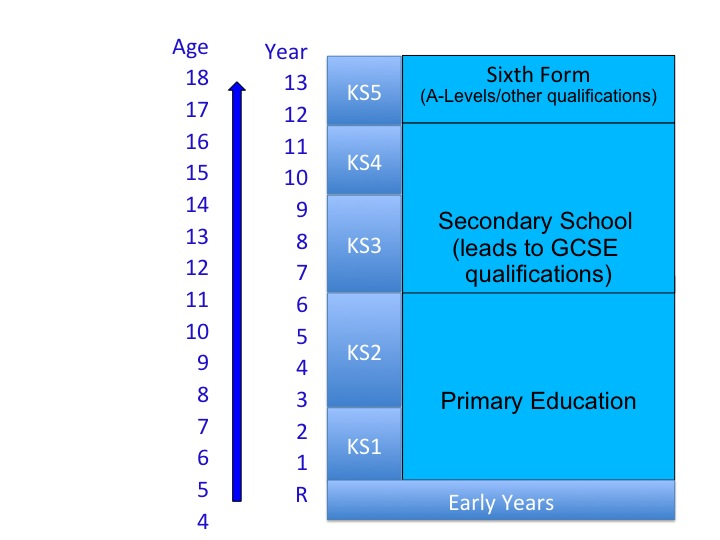
\includegraphics[width=\columnwidth]{images/key-stages.png}
  \caption{Key Stages in the English and Welsh education system}
  \label{fig:key-stages}
\end{figure}

% adjust to be Wales-focused
There is state provision for education in the UK up to the age of 19,
with mostly comprehensive, mixed ability schools across the UK. A few
areas in England have retained a system of selective 11+ schools
called grammar schools, which require students to sit an exam prior to
entry, but these schools are in the minority. As well as state
schools, 10\% of schools in the UK are independent fee-paying
schools. Overall, in England there are approximately 24,000 schools,
including 16,800 primary schools, 3,400 secondary schools and 2,400
independent schools (primary and secondary).  However, the primary and
independent schools tend to be smaller: the state-funded schools had
4.2 million primary pupils and 3.2 million secondary pupils, with 0.6
million pupils in independent schools. The ICT
curriculum in Wales
(2008)\footnote{\url{http://wales.gov.uk/topics/educationandskills/schoolshome/curriculuminwales/arevisedcurriculumforwales/nationalcurriculum/ictnc/?lang=en}},
was perceived to be less prescriptive than the ICT curriculum in
England, but exhibiting many of the same issues. It was recently
reviewed by an independent steering group appointed by the Welsh
Government~\cite{welshictreview:2013}, making clear recommendations for
reforming the ICT curriculum as part of a broader national curriculum
review for September 2014.

\section{The Technocamps Effect}

Technocamps is a multi-faceted Universities-based
operation engaging with schools -- both their pupils and their teachers --
throughout Wales and across all ages. Its main activities are as follows.

\begin{description}
\item[Workshops]
One-day campus-based workshops offered to whole classes
to give the pupils an introduction to computing,
particularly computational thinking and problem solving.
The whole class approach allows us: to address the gender divide,
by engaging with an equal number of boys and girls;
and to engage with those with no predisposition (or indeed an aversion)
to digital technology, to create an interest of computing within them.
\item[Technoclubs]
Lunchtime clubs in schools where pupils develop
their computational thinking and building skills.
\item[Bootcamps]
Two-day campus-based workshops held during school holidays.
\item[After Schools Clubs]
Two-hour late afternoon sessions held on campus or in the community.
\item[Playground Computing]
Day-long in-school workshops which present
the fundamentals of computer science to primary school pupils
through playful activities which develop computational thinking
and problem solving skills, but do not involve computers.
\item[Technoteach]
Training sessions, typically in the form of 20-hour modules
delivered one evening per week over six weeks.
Technoteach also encompasses other standalone twilight sessions
as well as an annual teachers conference.
\item[NEET Engagement]
Week-long summer residential sessions run in partnership with
the municipal youth services in which young people identified
as NEET (Not in Employment, Education of Training)
carry out a variety of team-building exercises,
learn app development and compete to design and build the best app.
\item[Student Placements]
Computer Science students at the University are offered
the opportunity to gain university course credits through
placements -- one day per week -- as teaching assistants
in school computing/ICT classes.
\end{description}

All Technocamps activities are provided completely free of charge
for all of its participants. This represents a huge investment
on the part of the Universities, but Technocamps has also received
various sources of funding in support of its activities.
The main funders are as follows.
\begin{description}
\item[ESF] (October 2010 - September 2014) --
A four-year \pounds 6 million EU-funded project to engage with secondary schools across South West Wales and the Valleys. This project involved Technocamps hubs at Aberystwyth University, Bangor University and the University of South Wales Glamorgan. Some 9,000 pupils from more than 180 schools and colleges have benefited from this project, as well as their teachers.
\item[NESTA] (June 2013 - December 2014) --
An 18-month \pounds 46,000 project to support the Playground Computing programme. This funding allows for a teacher to be seconded for 18 months to Technocamps in order to go out to primary schools throughout South Wales every day to present workshops. It has seen some 5,000 pupils at over 50 primary schools enjoy multiple day-long visits.
\item[National Science Academy] (November 2013 - March 2015) --
A 17-month \pounds 24,000 project to support the Technoteach programme; this funding was mainly in support of teachers registering on our six-week Technoteach modules, specifically providing their schools an amount of teacher cover to facilitate their attendance on the module. Over 120 teachers have thus far benefited from this project.
\item[Welsh Government] (September 2014 - March 2016) --
An 18-month \pounds 370,000 project under the Welsh Government's Learning in Digital Wales (LiDW) Tender. The LiDW Tender is to deliver 3-hour taster sessions at each of the 210 state-sponsored secondary schools across Wales, and will be delivered by each of the six Technocamps hubs.
\end{description}

\section{Conclusions}
End here...


% bib
\bibliographystyle{abbrv}
\bibliography{wipsce2015}


\section*{To Do}

In no particular order...

\begin{itemize}
\item Set UK context over past 3-5 years
\item Link to English and Scottish changes
\item Welsh context
\item Technocamps: the ten year journey from 2003
\item Convergence, the pan-Wales problem
\item Key contributions: aims, targets, impacts, young people, NEETs, coverage
\item Links with CAS Wales
\item Hubs (both TC and CAS)
\item Funding models: ESF, NSA, Nesta, etc
\item {\textbf{Key theme}}: Building capacity, the problems of
  England's NoE model in Wales
\item UK policy: RS report, English curriculum, qualification change,
  UKForCE, etc.
\item Welsh policy: ICT curriculum, ICT review, Estyn reports, ICT
  sector support/economic drivers, curriculum change,
  Donaldson and post-Donaldson
\item THE FUTURE...!
\end{itemize}

\subsection*{References to fit in}
\begin{itemize}
\item
General CAS
citations~\cite{crick+sentance:2011,brown-et-al-sigcse2012,brown-et-al-toce2014}.

\item
Teachers, CPD and
NoE~\cite{sentance-et-al-wipsce2012,sentance-et-al:2013,sentance-et-al:2014}.

\item
Technocamps~\cite{ball-et-al:2012,boyle-et-al:2012}

\item
Welsh Government report:
\begin{itemize}
\item
ICT Review~\cite{welshictreview:2013}
\item
Graham Report on STEM~\cite{STEMreview:2014}
\item
Donaldson Report~\cite{Donaldson:2015}
\item
Furlong Report~\cite{Furlong:2015}
\end{itemize}

\item
Misc Reports
\begin{itemize}
\item
NESTA Report~\cite{NESTA:2015}

\end{itemize}
\end{itemize}

\end{document}
